\chapter{Connectomes variations and  robustness}\label{ch:SC_indepth}

All the presented results up to this point (with an exception in Chapter \ref{ch:ftract}) were obtained with structural connectivity matrices created using Rosen and Halgren's averaging method from Mica-Mics dataset. Let us look closer at the possible group-averaging methods and possible variations in structural matrices based on the data source and group-averaging methods. 

\section{Minimal number of streamlines}

Having a structural connectivity matrix containing streamline counts as described in Section \ref{sec:edge_estimation}, we have to decide if it is enough to have one streamline connecting two regions to consider it as an edge. For example, Seguin et al. \cite{seguin_communication_2023} decided to prune connections comprising fewer than 5 streamlines. They justify this step with the high false positive rate of probabilistic tractography. Following their example, we did the same. In all the following group-averaging methods, we first discarded subject-level edges with less than 5 streamlines.

\section{Group-average structural connectome construction}\label{sec:group-avg}

Assume we already have a connectivity matrix for each subject in some group, edge weights representing streamline count. Because we want to work with the general structural properties of the brain, the question of constructing a group-representative connectome arises. Group averaging aims to increase the signal-to-noise ratio and obtain a clearer picture of brain network organization in general while preserving network properties that are consistently expressed at the subject level (such as edge length distribution). \cite{betzel_distance-dependent_2019} In this section, we present some possible approaches.

\subsection{Simple average}\label{sec:average}

The most straightforward idea is to average the streamline count between each pair of nodes across all the subjects. The main problem with this approach is that whenever there is at least one subject with an edge from A to B, the AB average is always non-zero, suggesting that \enquote{there is a connection between these nodes}. As a result, the network density might be higher in the averaged connectome. That is an issue, especially because the process of obtaining streamline counts is erroneous, and the presence of one subject with this edge might be an accident.

\subsection{Consensus thresholding}\label{sec:cons-thr}

Consensus thresholding is the most common approach. It tries to preserve features consistently expressed at individual subjects' level while reducing noise. Threshold $\tau$ between 0 and 1 is specified\footnote{There is no consensus about the \enquote{correct} value of $\tau$ and it is often selected according to some heuristics. That might be a source of complications while attempting to compare connectomes across different studies.}, and the connections that are observed in at least $\tau$ fraction of subjects are kept. These connections are associated with weight, for example, the average number of streamlines among the subjects where the connection is present. The rest is set to 0. \cite{betzel_distance-dependent_2019}

Betzel et al. point out that this approach favors shorter edges which are easier to reconstruct using tractograpy. Consequently, the distribution of edge lengths is different in average connectome than in the single subjects. According to their argumentation, the longer edges are less common, but despite that, they have an important function in the brain. On the grounds of that, it is important to keep the edge length distribution because structural networks need long-distance connections. They propose their own method to prevent the issue, and we present it below. \cite{betzel_distance-dependent_2019} 

\subsection{Distance-dependent consensus thresholding}\label{sec:dist-dep}

This method aims to preserve edge length distribution. Assume the list of edges and their lengths. \footnote{Lengths might be Euclidean distances of the nodes or some sort of streamline average lengths.} Let us define $M$ as the total number of edges we want to keep in the consensus network. We define $M$ bins based on edge length percentiles. For each of them, we find all possible edges falling into that bin by length. For each bin, we choose the edge that is expressed most often across the subjects with ties broken by the greatest average weight (for example, streamline count). \cite{betzel_distance-dependent_2019} 

We used \texttt{struct\_consensus} method from netneurotools package\footnote{\url{https://netneurotools.readthedocs.io/en/latest/index.html}} for Python for calculation of distance-dependent thresholding during the work on this thesis.

\subsection{Averaging by Rosen and Halgren}\label{sec:rh}

This method was used by Rosen and Halgren in the paper \textit{A Whole-Cortex Probabilistic Diffusion Tractography Connectome} \cite{rosen_whole-cortex_2021} in a group-averaging of the matrix described in Section \ref{sec:rhdata}.

The principle is the same as a simple average, but it works with a ratio of streamlines between two parcels to a global number of streamlines instead of plain streamline counts. According to the paper, the values are first averaged across the subjects and then scaled such as the number of streamlines originating at parcel A and terminating at parcel B is divided by the total number of streamlines that either originate at parcel A or terminate at parcel B, excluding within-parcel connections. \cite{rosen_whole-cortex_2021} We used the equation below, where $SC$ is the final structural connectivity matrix and $m$ is an average of structural matrices across individual subjects.

$$
SC_{ij} = \frac{m_{ij}}{\sum_k m_{ik} + \sum_l m_{lj} - (m_{ii} - m_{jj})}
$$

In practice, he resulting matrix was sometimes non-symmetric even if the individual subject matrices were symmetric. It was caused by numerical instability in Python while working with small numbers. To overcome this problem, we added $SC = (SC + SC^T) /2$ to the end of the procedure.

\section{Structural connectome density}

Seguin et al. \cite{seguin_communication_2023} in the paper \textit{Communication dynamics in the human connectome shape the cortex-wide propagation of direct electrical stimulation} propose one more step in connectome construction. They prune the group-averaged connectivity matrices keeping the edges with the highest weight such that the density of the connectome is 25\%. 

The density of structural connectivity matrices differs across da\-ta\-sets, it depends on the individual connectome construction parameters. For example, the average connection density in Mica-Mics dataset is  84.1\% across subjects. \cite{seguin_communication_2023} If we want to get comparable results, it is necessary to start with connectomes with similar density. Because of that, we decided to threshold all the group-average matrices and keep approximately 25\% strongest edges.\footnote{Seguin et al. thresholded the subject-level matrices, but we do not have those available for some of the datasets. Because of that, we decided to do this step later to get the same density for all structural connectivity matrices.}

\section{Structural connectomes description}

All structural connectomes used during our work are described in this section. Some of them were published as group-averaged, while others came as a set of single-subject matrices. This section presents how they were constructed and compares them. 

\subsection{Enigma}\label{sec:enigma}

The first source of structural connectivity matrices for this thesis is a Python package ENIGMA TOOLBOX\footnote{\url{https://enigma-toolbox.readthedocs.io/en/latest/}, accessed 1. 5. 2024} developed by S. Larivière and B. Bernhardt from MICA Lab - Montreal Neurological Institute \cite{lariviere_enigma_2020}. It provides an option to load structural connectivity matrices in several parcellations. The original data were taken from 207 healthy adults from the HCP dataset.\footnote{The Human Connectome Project (HCP) is a large scientific effort focused on mapping the connectivity of the human brain. The HCP datasets are openly available to researchers at \url{https://www.humanconnectome.org/}. \cite{van_essen_human_2012}} The preprocessing pipeline is described in detail in a paper \textit{The ENIGMA Toolbox: Cross-disorder integration and multiscale neural contextualization of multisite neuroimaging datasets} by Larivière et al. For our application, it is important to note that the group average structural connectome was obtained using a distance-dependent thresholding procedure described above~\ref{sec:dist-dep}. Afterward, it was log-transformed. The structural connectomes are available in DK, Glasser, and Schaefer parcellations. 

There is a disadvantage of Enigma structural matrices, they provide only edge weights, not lengths. It is also important to mention that for Glasser and Schaefer parcellations, there are no zero weights in the matrix, but most of it is filled with ones (which is not the case for the DK parcellation) -- connectome is a complete graph with weights mostly one.

\subsection{Domhof}\label{sec:domhof}

This dataset, created by Domhof et al. \cite{domhof_parcellation-based_2022}, is available online on the EBRAINS platform.\footnote{\url{https://doi.org/10.25493/NVS8-XS5}} The repository provides individual connectomes for 200 subjects from the Human Connectome Project (HCP). For each subject, there is a matrix with streamline counts and a matrix with streamline lengths. They provide the connectomes in 20 different parcellations, including DK and Schaefer200 parcellations. 

During the data exploration, we found that there are 70 ROIs in the matrices in the DK parcellation. We removed the surplus ROIs to achieve compatibility with Enigma.

We constructed the group-representative matrices using three approaches described in Section~\ref{sec:group-avg}, namely simple average, distance-dependent consensus thresholding, and the Rosen and Halgren method. For streamline lengths group average, we calculated an average considering only the values for which the corresponding weight was non-zero.

\subsection{Mica-Mics}\label{sec:mica}

This dataset was published by Royer et al. \cite{royer_open_2021} on The Canadian Open Neuroscience Platform.\footnote{\url{https://n2t.net/ark:/70798/d72xnk2wd397j190qv}} It consists of multimodal data from 50 healthy adult subjects and there are Glasser and Schaefer200 parcellations available. We constructed the group-representative matrices for both of them using the same approaches as for the Domhof dataset.

\subsection{RosenHalgren}\label{sec:rhdata}

This dataset was published by Rosen and Halgren. \cite{rosen_whole-cortex_2021} It is again based on data from HCP, this time 1065 healthy adults. The group representative weights and lengths matrices are available on Zenodo\footnote{\url{https://doi.org/10.5281/zenodo.10150880}} in Glasser parcellation. The group average was created following the averaging procedure described above. 

\subsection{PyTepFit}\label{sec:pytepdata}

The last structural connectivity weights and lengths matrices were taken from a GitHub repository\footnote{\url{https://github.com/GriffithsLab/PyTepFit/tree/66b94e488c82478e6f302015b6cd8e8d9d33792a/data}} of PyTepFit project by Momi~et~al. \cite{momi_tms-evoked_2023}. These are already group-averaged (simple average) matrices with Schaefer200 parcellation created using data from 400 healthy subjects from the HCP project. 

\section{Structural connectomes comparison}

This work aims to investigate the relationship between structural connectivity and brain function. Before we move to that in Chapter~\ref{ch:ftract} and Chapter~\ref{ch:pytepfit}, we should explore the structural connectivity itself. It is necessary to understand the nature of structural connectivity and how it differs depending on the data source and preprocessing method before we use it to predict the function. The previous sections described where the structural matrices come from and what they represent. Now, let us focus on the differences between various preprocessing methods introduced in Section~\ref{sec:group-avg}.

In this section, we chose the Schaefer200 parcellation to present the results because we have the most data available in this parcellation. \TODO[jiné parcelace]

\subsection{Overall comparison}

In the following chapters, we investigate correlations between the structure and function. It raises the question of what the correlations are between matrices of structural connectivity weights themselves.\footnote{We calculated the lengths in the same way for all preprocessing methods, so we do not compare lengths here.} We are interested in Spearman correlations later, so we discuss the Spearman correlation coefficient here for consistency. The results are shown in the Figure~\ref{fig:sc_correlations}. 

Regardless of the preprocessing method, there are higher correlations between Domhof and Mica-Mics matrices than the others. Within these datasets, we see that in our setting there is basically no difference between simple average and consensus thresholding. This is because the original individual-subject matrices are dense, so the probability that there is an edge in many of the subjects is high. It also holds for both Domhof and Mica-Mics datasets that the matrix created using a distance-dependent consensus thresholding method has the lowest correlations with the others.

\begin{figure}[p]
  \begin{center}
    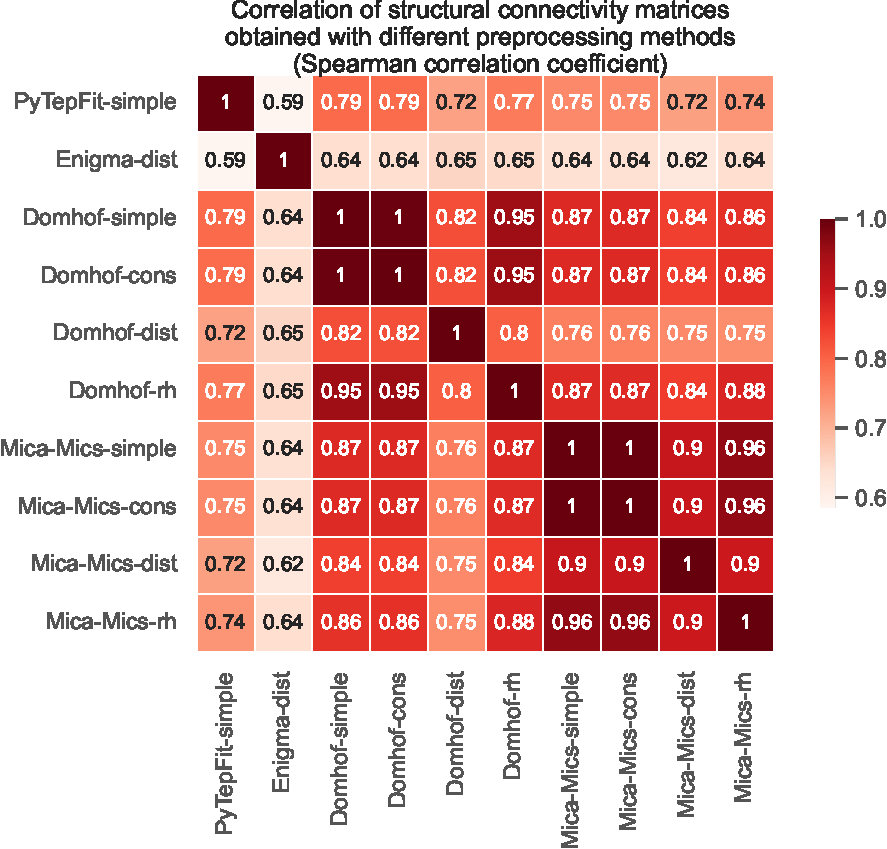
\includegraphics[width=\textwidth]{images/nootebook_generated/sc_comparison/schaefer/5/0.25/correlations_all_matrices_Spearman.pdf}
  \end{center}
  \caption[Correlations of SC matrices (Schaefer200 parcellation)]{Spearman correlations ($p<0.05$ for all results) of structural connectivity matrices with Schaefer200 parcellation. }
  \label{fig:sc_correlations}
\end{figure}


\subsection{Distribution of edge weights}

Another question is if the preprocessing method influences the distribution of edge weights. We can see in Figure~\ref{fig:edge_weights_schaefer} for the Mica-Mics dataset that the simple average is again nearly the same as consensus thresholding, and they both result in a higher number of weaker edges than Rosen and Halgren's. Rosen and Halgren's method yields proportionally a higher number of stronger edges than the other methods. The results for the Domhof dataset look similar, only the distribution for distance-dependent consensus thresholding is slightly shifted to the higher weights.

However, there is a difference if we look at different parcellations. Figure~\ref{fig:edge_weights_glasser} differs from~\ref{fig:edge_weights_schaefer} only in the parcellation, but there are much bigger differences in the edge weights distributions based on the preprocessing method. Especially there is a difference between simple average and consensus thresholding, the former having a higher number of weaker edges. Rosen and Halgren's method still gives a higher number of stronger edges than the other methods, and the effect is even more visible in this case.

The reason for the difference between the parcellations is probably caused by their different granularity. Let us remind you that Schafer200 has 200 ROIs, while Glasser 360. We use the same DW-MRI data as a basis for connectomes with both parcellations. In the case of finer parcellation, the resulting connectome may exhibit lower density. This is because if there are only a few streamlines connecting certain ROIs, further subdivisions of these regions could lead to the absence of streamlines between some pairs of ROIs in the subdivision. Therefore there are more zeros in the connectivity matrices for individual subjects for Glasser parcellation. Because of that, there is a higher number of weaker edges in the simple group average because we are averaging the zeros as well. \footnote{The effect is there even if the density is the same as for the consensus thresholding method because we are averaging only the non-zero values during the consensus thresholding connectome calculation.}

\begin{figure}[p]
\begin{subfigure}{\textwidth}
      \begin{center}
    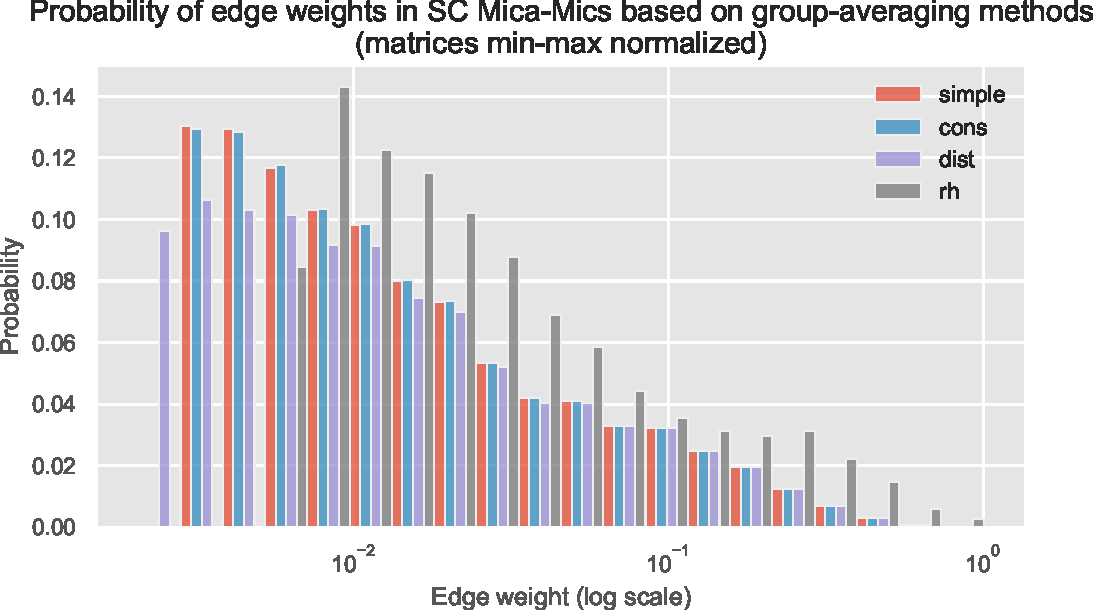
\includegraphics[width=\textwidth]{images/nootebook_generated/sc_comparison/schaefer/5/0.25/Probability_of_edge_weights_in_SC_Mica-Mics_based_on_group-averaging_methods_(matrices_min-max_normalized).pdf}
  \end{center}
  \caption{Schaefer200 parcellation}
  \label{fig:edge_weights_schaefer}
\end{subfigure}

\bigskip

\begin{subfigure}{\textwidth}
      \begin{center}
    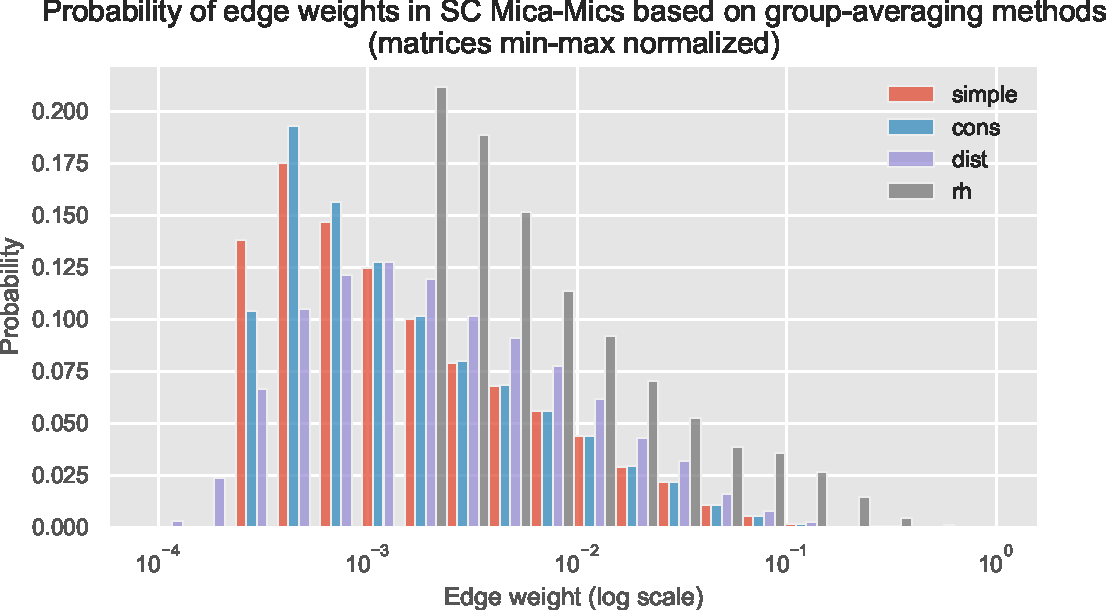
\includegraphics[width=\textwidth]{images/nootebook_generated/sc_comparison/MNI-HCP-MMP1/5/0.25/Probability_of_edge_weights_in_SC_Mica-Mics_based_on_group-averaging_methods_(matrices_min-max_normalized).pdf}
  \end{center}
  \caption{Glasser parcellation}
  \label{fig:edge_weights_glasser}
\end{subfigure}
\caption[Edge weights distribution per preprocessing method]{Edge weights distribution per preprocessing method for Mica-Mics dataset and Schaefer200 and Glasser parcellations. All matrices were min-max normalized because the weights of the rh method are not comparable with the others otherwise. The y-axis shows a probability (not count) for better comparability because the number of edges differs for the \texttt{dist} method.}
\end{figure}

\begin{figure}[p]
  \begin{center}
    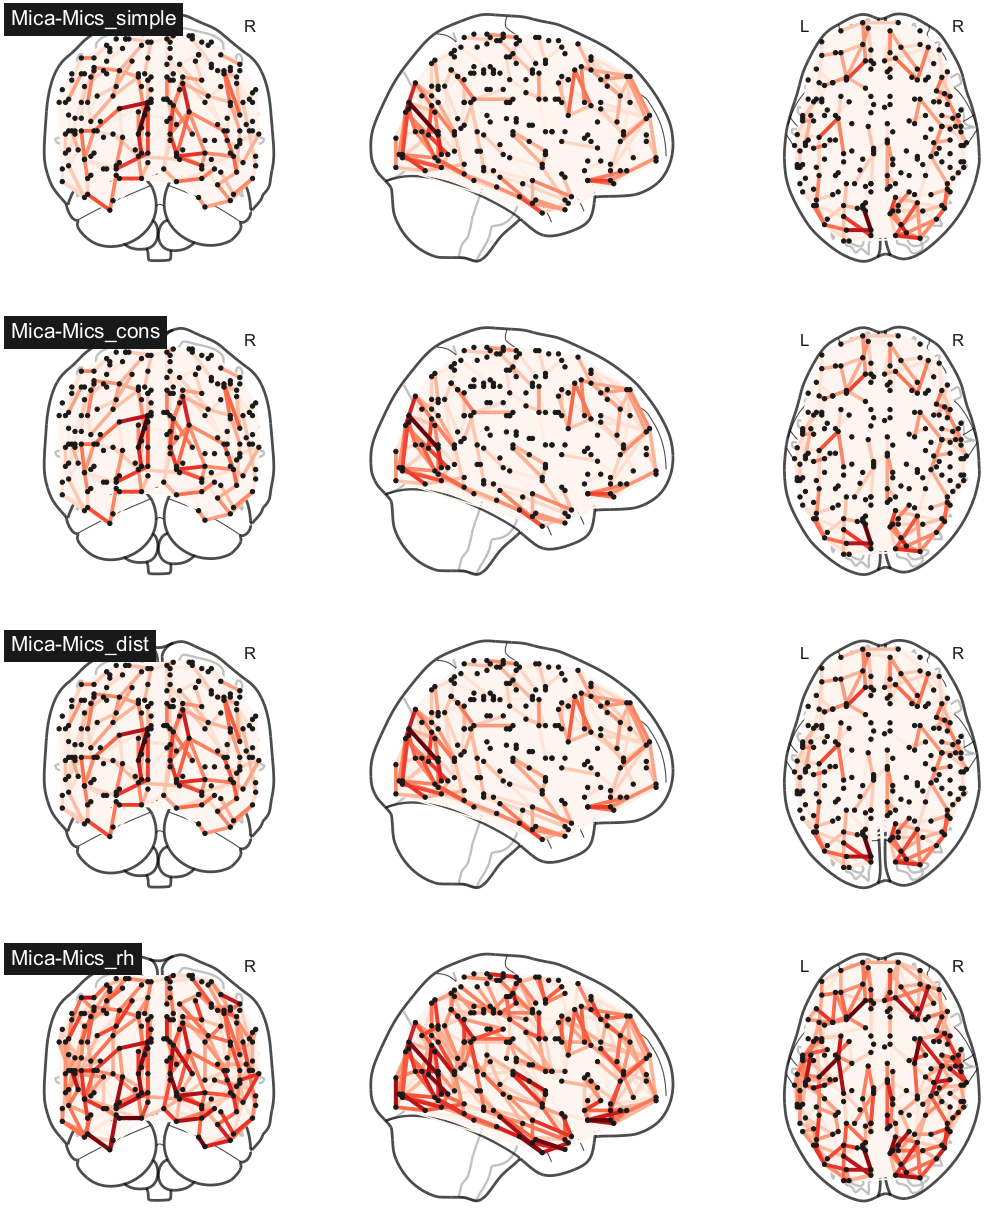
\includegraphics[width=\textwidth]{images/manually_created/mica.png}
  \end{center}
  \caption[Connectomes based on preprocessing method]{Connectomes based on group-averaging method (simple averaging, consensus thresholding, distance dependent consensus threshodling and Rosen and Halgren's method) for Schaefer200 parcellation, Mica-Mics dataset, edge weights log-transformed and min-max normalized. In a common color scale, a darker color denotes stronger edges.}
  \label{fig:connectomes_mica}
\end{figure}

\begin{figure}
\begin{center}
    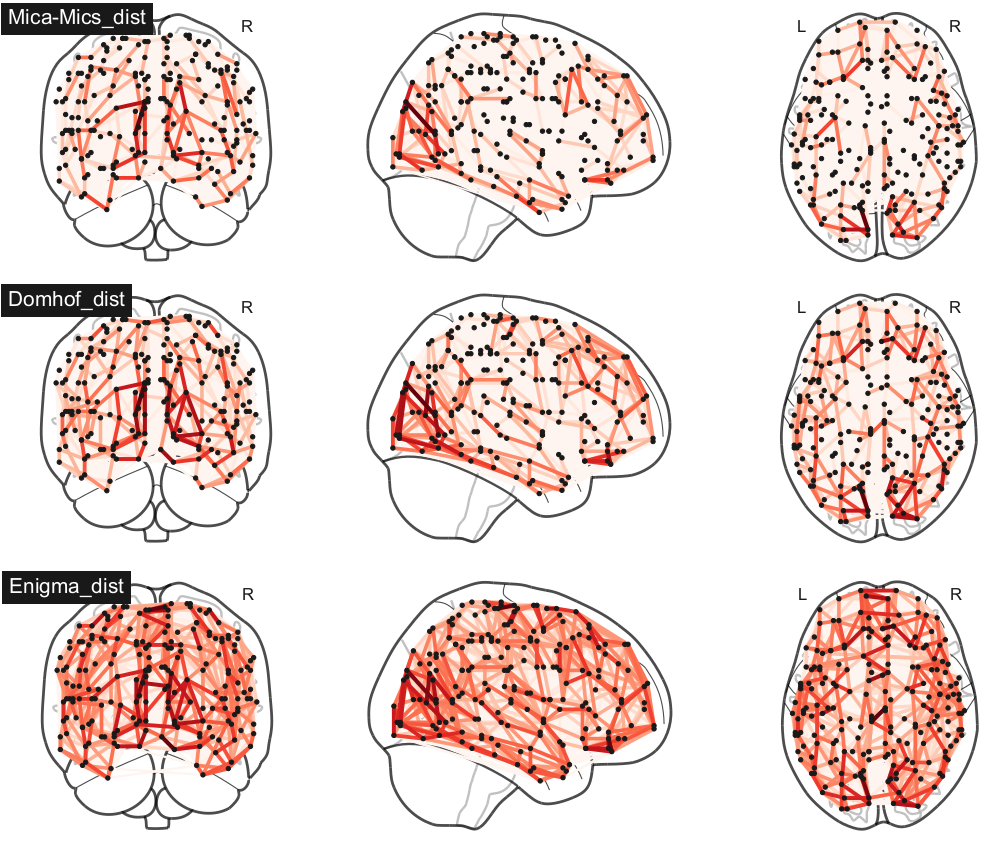
\includegraphics[width=0.9\textwidth]{images/manually_created/datasets.png}
  \end{center}
  \caption[Connectomes based on dataset]{Connectomes based on dataset (Mica-Mics, Domhof, and Enigma) for Schaefer200 parcellation, edge weights log-transformed and min-max normalized. All datasets group averaged using distance dependent consensus thresholding method. In a common color scale, a darker color denotes stronger edges.}
  \label{fig:connectomes_by_dataset}
\end{figure}

We were also curious if the distribution of edge weights in the brain differs based on the preprocessing method. Figure~\ref{fig:connectomes_mica} shows the edge weights in the brain for different preprocessing methods. It is already discussed above and shown in Figure~\ref{fig:edge_weights_schaefer} that different preprocessing methods yield different numbers of stronger edges. Besides that, Rosen and Halgren's group averaging method creates a slightly different structure than the others. However, the structure of the connectome weights differs much more based on the datasets. See Figure \ref{fig:connectomes_by_dataset}. 

\subsection{Distribution of edge lengths}

We mention in Section~\ref{sec:dist-dep} that the primary reason for the introduction of the distance-dependent thresholding method was to prevent the omission of long edges in group average connectomes. However, as shown in Figure~\ref{fig:edge_lengths}, our results do not confirm that the method fulfills this goal. Although there are slightly more longer edges for Schaefer200 parcellation, the differences in edge length distribution are really small and probably negligible. 

\begin{figure}[p]
\begin{subfigure}{\textwidth}
      \begin{center}
    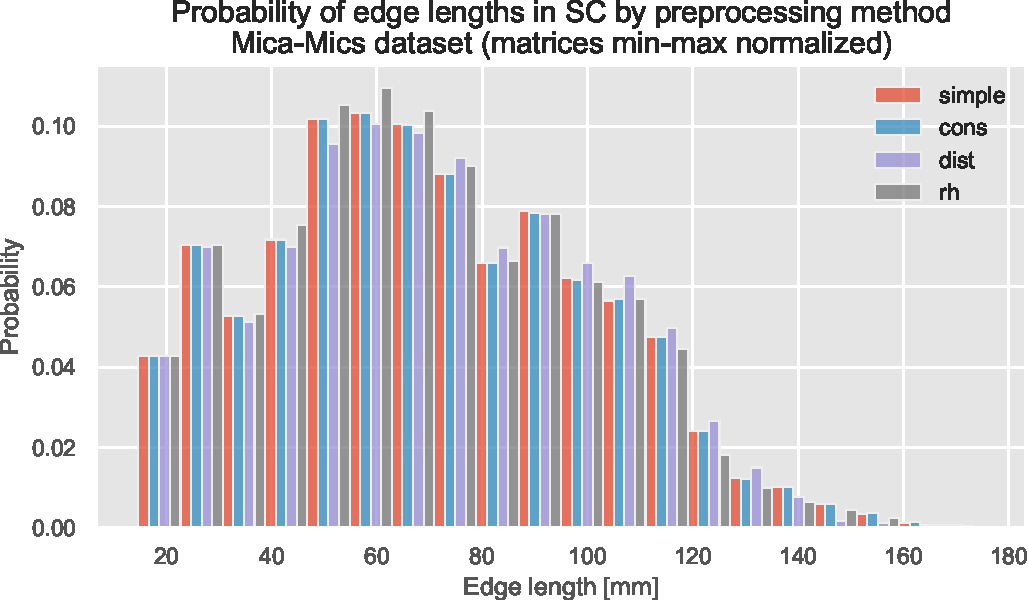
\includegraphics[width=\textwidth]{images/nootebook_generated/sc_comparison/schaefer/5/0.25/Probability_of_edge_lengths_in_SC_by_preprocessing_method_Mica-Mics_dataset_(matrices_min-max_normalized).pdf}
  \end{center}
  \caption{Schaefer200 parcellation}
  \label{fig:edge_lengths_schaefer}
\end{subfigure}

\bigskip

\begin{subfigure}{\textwidth}
      \begin{center}
    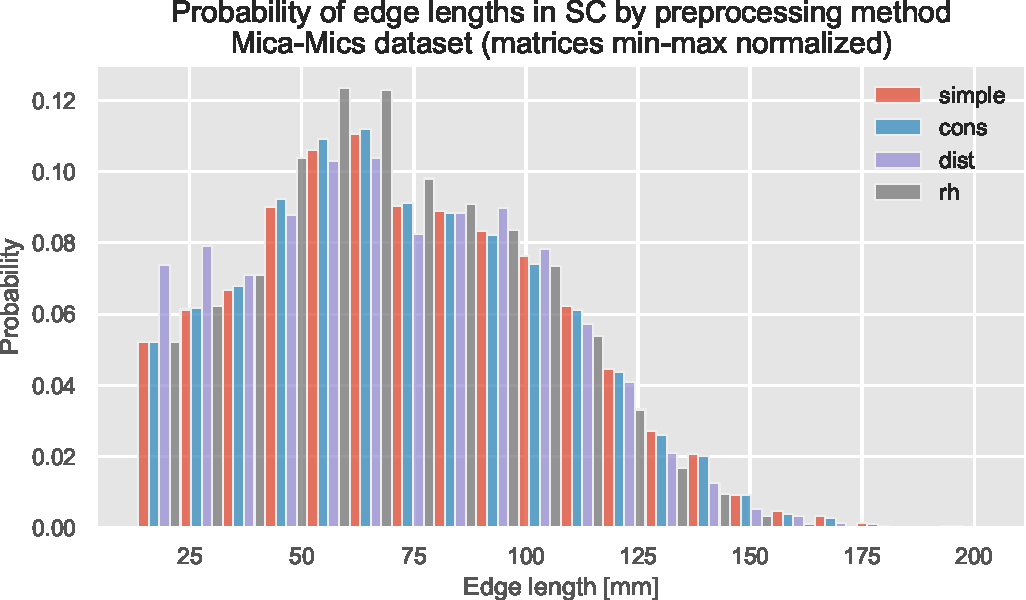
\includegraphics[width=\textwidth]{images/nootebook_generated/sc_comparison/MNI-HCP-MMP1/5/0.25/Probability_of_edge_lengths_in_SC_by_preprocessing_method_Mica-Mics_dataset_(matrices_min-max_normalized).pdf}
  \end{center}
  \caption{Glasser parcellation}
  \label{fig:edge_lengths_glasser}
\end{subfigure}
\caption[Edge lengths distribution per preprocessing method]{Edge lengths distribution per preprocessing method for Mica-Mics dataset and Schaefer200 and Glasser parcellations. The y-axis shows a probability (not count) for better comparability because the number of edges differs for the \texttt{dist} method.}
\label{fig:edge_lengths}
\end{figure}

\section{Robustness of the previous results}

Section \ref{sec:sc-robustness_ftract} already discussed the robustness of F-TRACT results to structural connectome selection. In this section, let us first discuss the results for F-TRACT obtained with Deskian-Killiany parcellation. Then, we move to TMS-EEG and look at the results with a different dataset or a group-averaging method.

\subsection{F-TRACT with Deskian-Killiany parcellation}

As mentioned in Section \ref{sec:parcellations}, the selection of parcellation can influence the results obtained later with the data. We illustrate the issue here. 

Figure  \ref{fig:ftract_alldata_long_probabilities_DK} shows that both full and partial correlations of response probability with structural connectivity and communication metrics are preserved with the change of parcellation from Glasser (360 regions) to Deskian-Killiany (68 regions), even when the results differ (for example, the highest correlation of response probability is with the structural connectivity for Deskian-Killiany, but with the shortest path efficiency for Glasser). However, Figure \ref{fig:ftract_alldata_long_amplitudes_DK} shows that for the amplitudes, there are no significant correlations when the Deskian-Killiany parcellation is used.

\begin{figure}
    \centering
    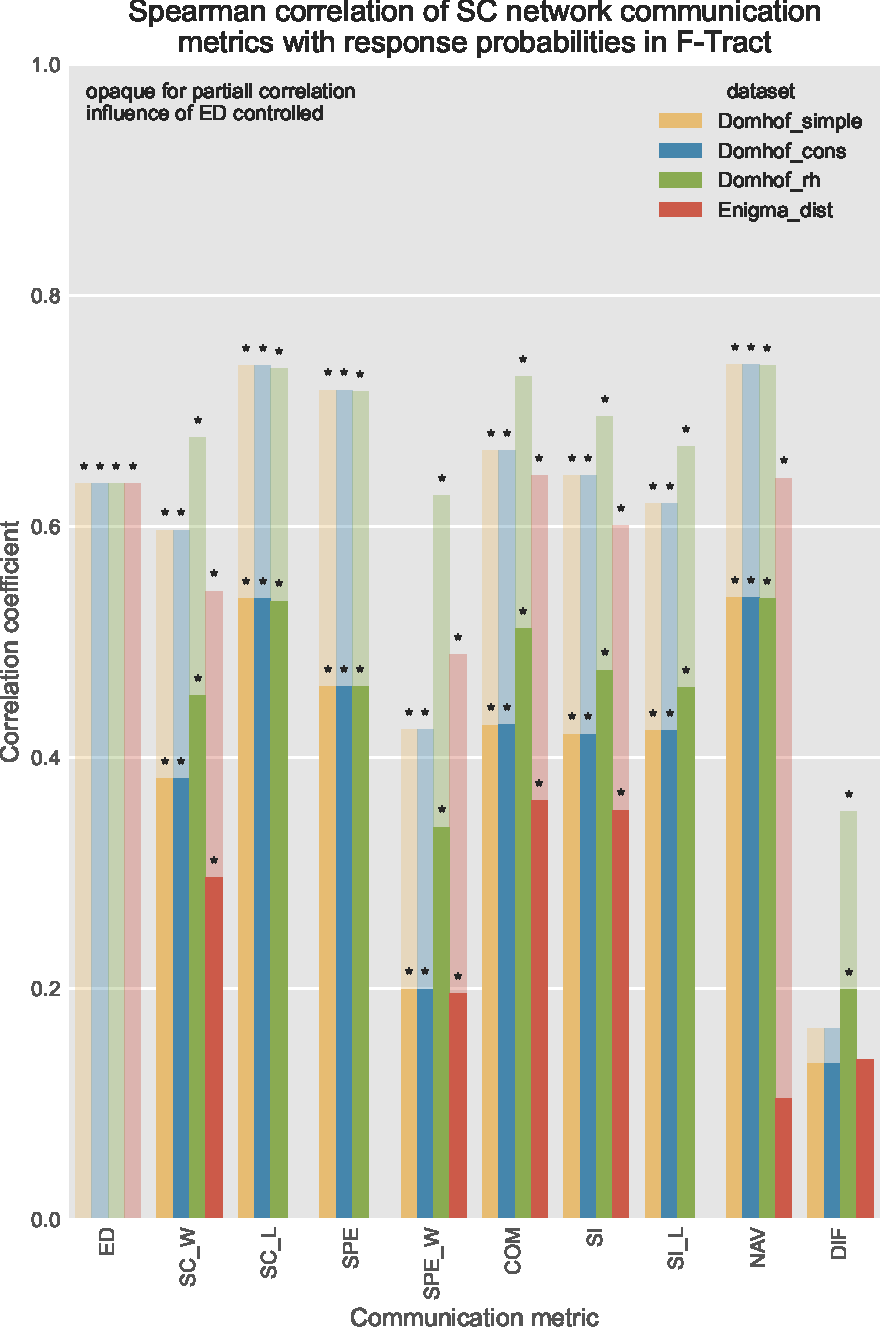
\includegraphics[width=0.93\textwidth]{images/nootebook_generated/ftract_results/DKT/5/ED0/0.25/long/Spearman_correlation_of_SC_network_communication_metrics_with_response_probabilities_in_F-Tract.pdf}
    \caption[F-TRACT probability correlations - all $SC$ matrices (DK)]{Correlations (absolute value) of response probability (200~ms response) and structural connectivity and derived communication metrics (DK parcellation). Asterisks denote a significant correlation ($p<0.05$).}
    \label{fig:ftract_alldata_long_probabilities_DK}
\end{figure}

\begin{figure}
    \centering
    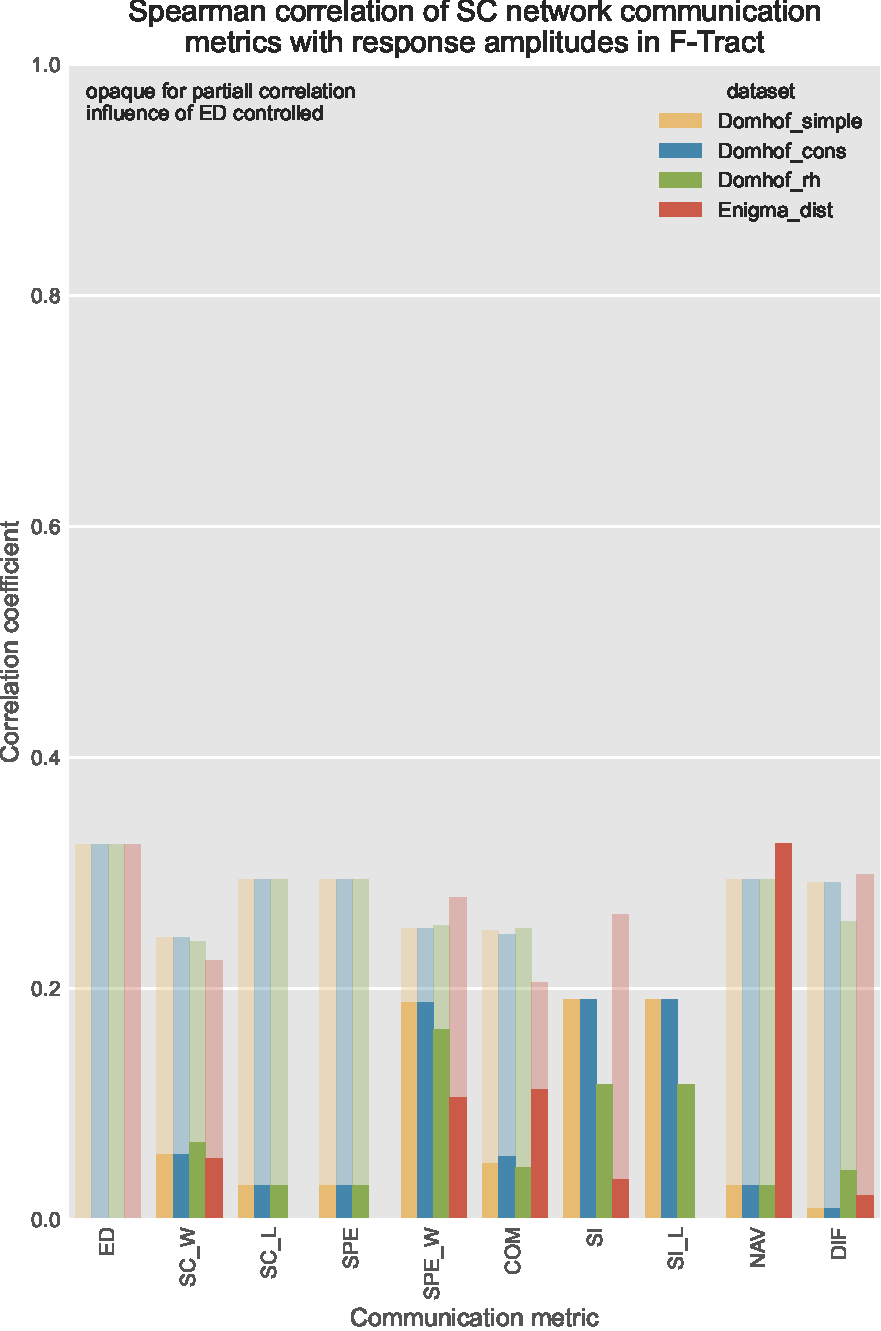
\includegraphics[width=0.93\textwidth]{images/nootebook_generated/ftract_results/DKT/5/ED0/0.25/long/Spearman_correlation_of_SC_network_communication_metrics_with_response_amplitudes_in_F-Tract.pdf}
    \caption[F-TRACT amplitude correlations - all $SC$ matrices (DK)]{Correlations (absolute value) of response amplitude (200~ms response) and structural connectivity and derived communication metrics (DK parcellation). Asterisks denote a significant correlation ($p<0.05$)}
    \label{fig:ftract_alldata_long_amplitudes_DK}
\end{figure}

\subsection{TMS-EEG with different datasets and group-averaging methods}

We tried to calculate the results from Section \ref{sec:results_pytepfit-empirical} with different datasets and group-averaging methods for the 200 ms responses as a control.  

Regarding the group-averaging method, we tried all the methods described in Section \ref{sec:group-avg}. We applied them to the Mica-Mics dataset. There are no differences in the results obtained with simple averaging, consensus thresholding, and Rosen and Halgren's method. The results obtained with distance-dependent consensus thresholding preserve the important features like high correlation of response characterized by AUC with the shortest path efficiency and the navigation efficiency (Figure \ref{fig:tms_auc_200_dist}, compare with Figure \ref{fig:tms_auc_200}), but there are differences, for example, overall lover or non-significant correlations for binarized responses (Figure \ref{fig:tms_01_200_dist}, compare with Figure \ref{fig:tms_01_200}).

\begin{figure}
    \centering
    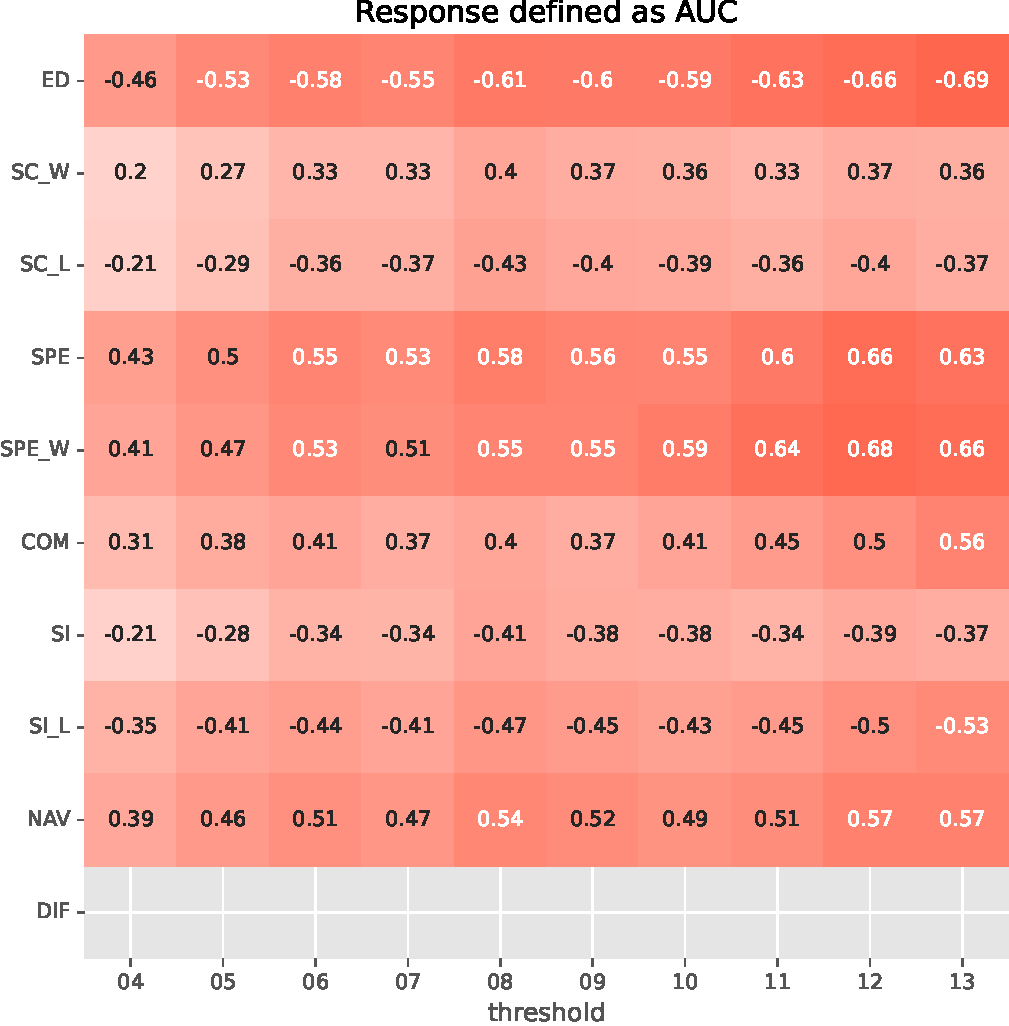
\includegraphics[width=\textwidth]{images/nootebook_generated/pytepfit_results/empirical/200/not_over_threshold_nan/Mica-Mics_dist/Response defined as AUC.pdf}
    \caption[TEPs AUC (200 ms) correlations (dist)]{Spearman correlation coefficient of AUC of empirical TEP (200 ms response) with structural connectivity and communication metrics. Darker color denoted a higher absolute value of the correlation; missing values are non-significant ($p>0.05$). Group averaging method: distance-dependent consensus thresholding.}
    \label{fig:tms_auc_200_dist}
\end{figure}

\begin{figure}
    \centering
    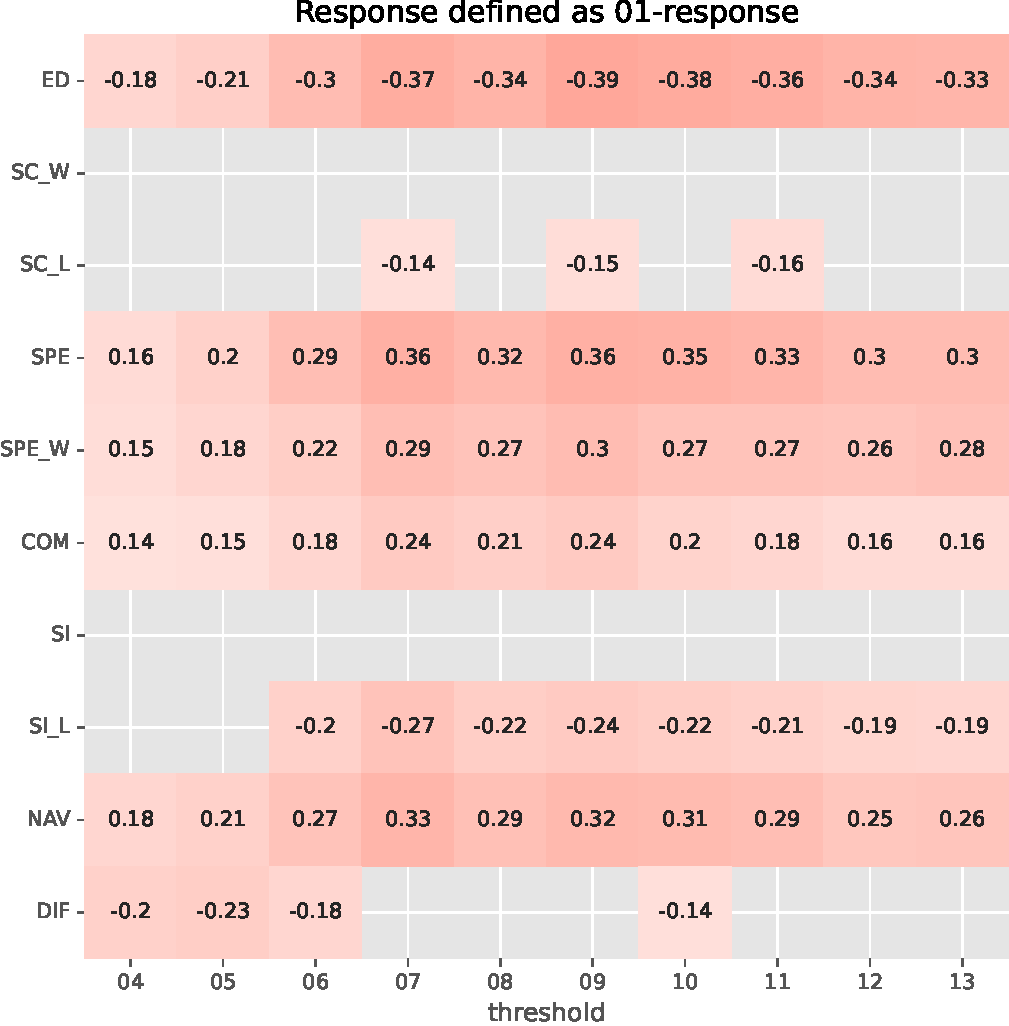
\includegraphics[width=\textwidth]{images/nootebook_generated/pytepfit_results/empirical/200/not_over_threshold_nan/Mica-Mics_dist/Response defined as 01-response.pdf}
    \caption[Binarized TEP (200 ms) correlations (dist)]{Spearman correlation coefficient of binarized empirical TEP (200 ms response) with structural connectivity and communication metrics. Darker color denoted a higher absolute value of the correlation; missing values are non-significant ($p>0.05$). Group averaging method: distance-dependent consensus thresholding.}
    \label{fig:tms_01_200_dist}
\end{figure}

Regarding the dataset, we tried Enigma \ref{sec:enigma}, Domhof \ref{sec:domhof}, and PyTepFit \ref{sec:pytepdata} datasets. The results slightly differ for all of them, but the key features discussed in Section \ref{sec:results_pytepfit-empirical} are always present: AUC and the first peak time correlate with communication metrics, and the highest correlations are achieved for the shortest path efficiency and navigation efficiency. See Figure \ref{fig:tms_auc_200_pytep_simple} showing results for PyTepFit dataset and response characterized by AUC as an illustrative example (compare with Figure \ref{fig:tms_auc_200}).

\begin{figure}
    \centering
    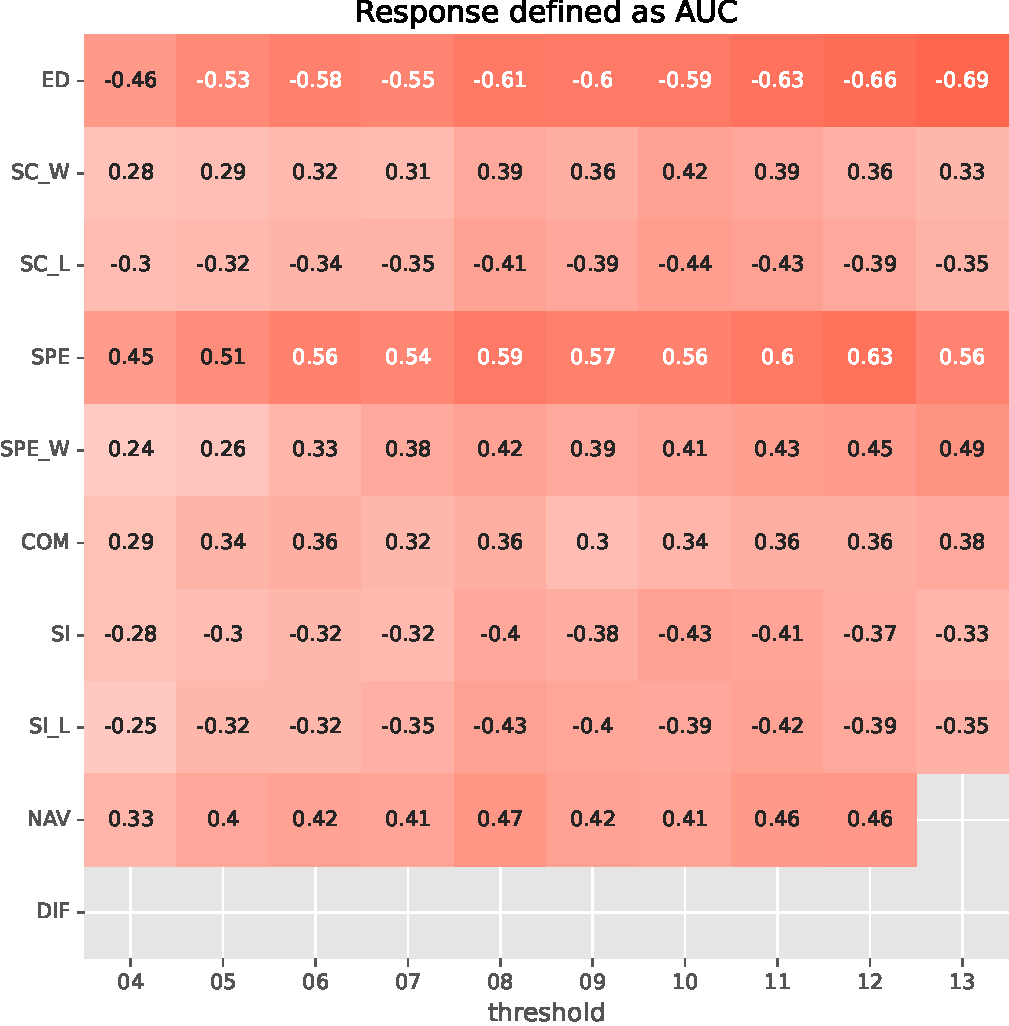
\includegraphics[width=\textwidth]{images/nootebook_generated/pytepfit_results/empirical/200/not_over_threshold_nan/PyTepFit_simple/Response defined as AUC.pdf}
    \caption[TEPs AUC (200 ms) correlations (PyTepFit)]{Spearman correlation coefficient of AUC of empirical TEP (200 ms response) with structural connectivity and communication metrics. Darker color denoted a higher absolute value of the correlation; missing values are non-significant ($p>0.05$). Group averaging method: simple averaging, dataset: PyTepFit.}
    \label{fig:tms_auc_200_pytep_simple}
\end{figure}


\section{Conclusion}

The main takeaway of this section is, that the choice of a dataset, parcellation, and preprocessing method has an impact on the resulting connectome. Consequently, the connectome has an impact on the results of subsequent analysis.

First of all, the different data sources might differ in the measurement settings, DW-MRI preprocessing, and many other aspects along the way from the human brain to the connectivity matrix. With Figure \ref{fig:sc_correlations} and Figure \ref{fig:connectomes_by_dataset} in mind, we recommend using structural connectivity matrices from different sources whenever possible because they could differ quite a lot.

The choice of parcellation is an important step as well. We aim to use graph theoretical metrics to get better insight into the brain function, and the number of nodes (not mentioning other differences of the parcellations) could have a great impact on the subsequent analysis.

Even though there are differences in the connectomes and consequently in the results, we confirmed that the observations from Chapters \ref{ch:ftract} and \ref{ch:pytepfit} are robust regarding the connectome selection.